% !TeX spellcheck = it_IT
\section{Long Term Evolution 4G LTE}

Confronto tra architettura 3G e 4G:
\begin{center}
	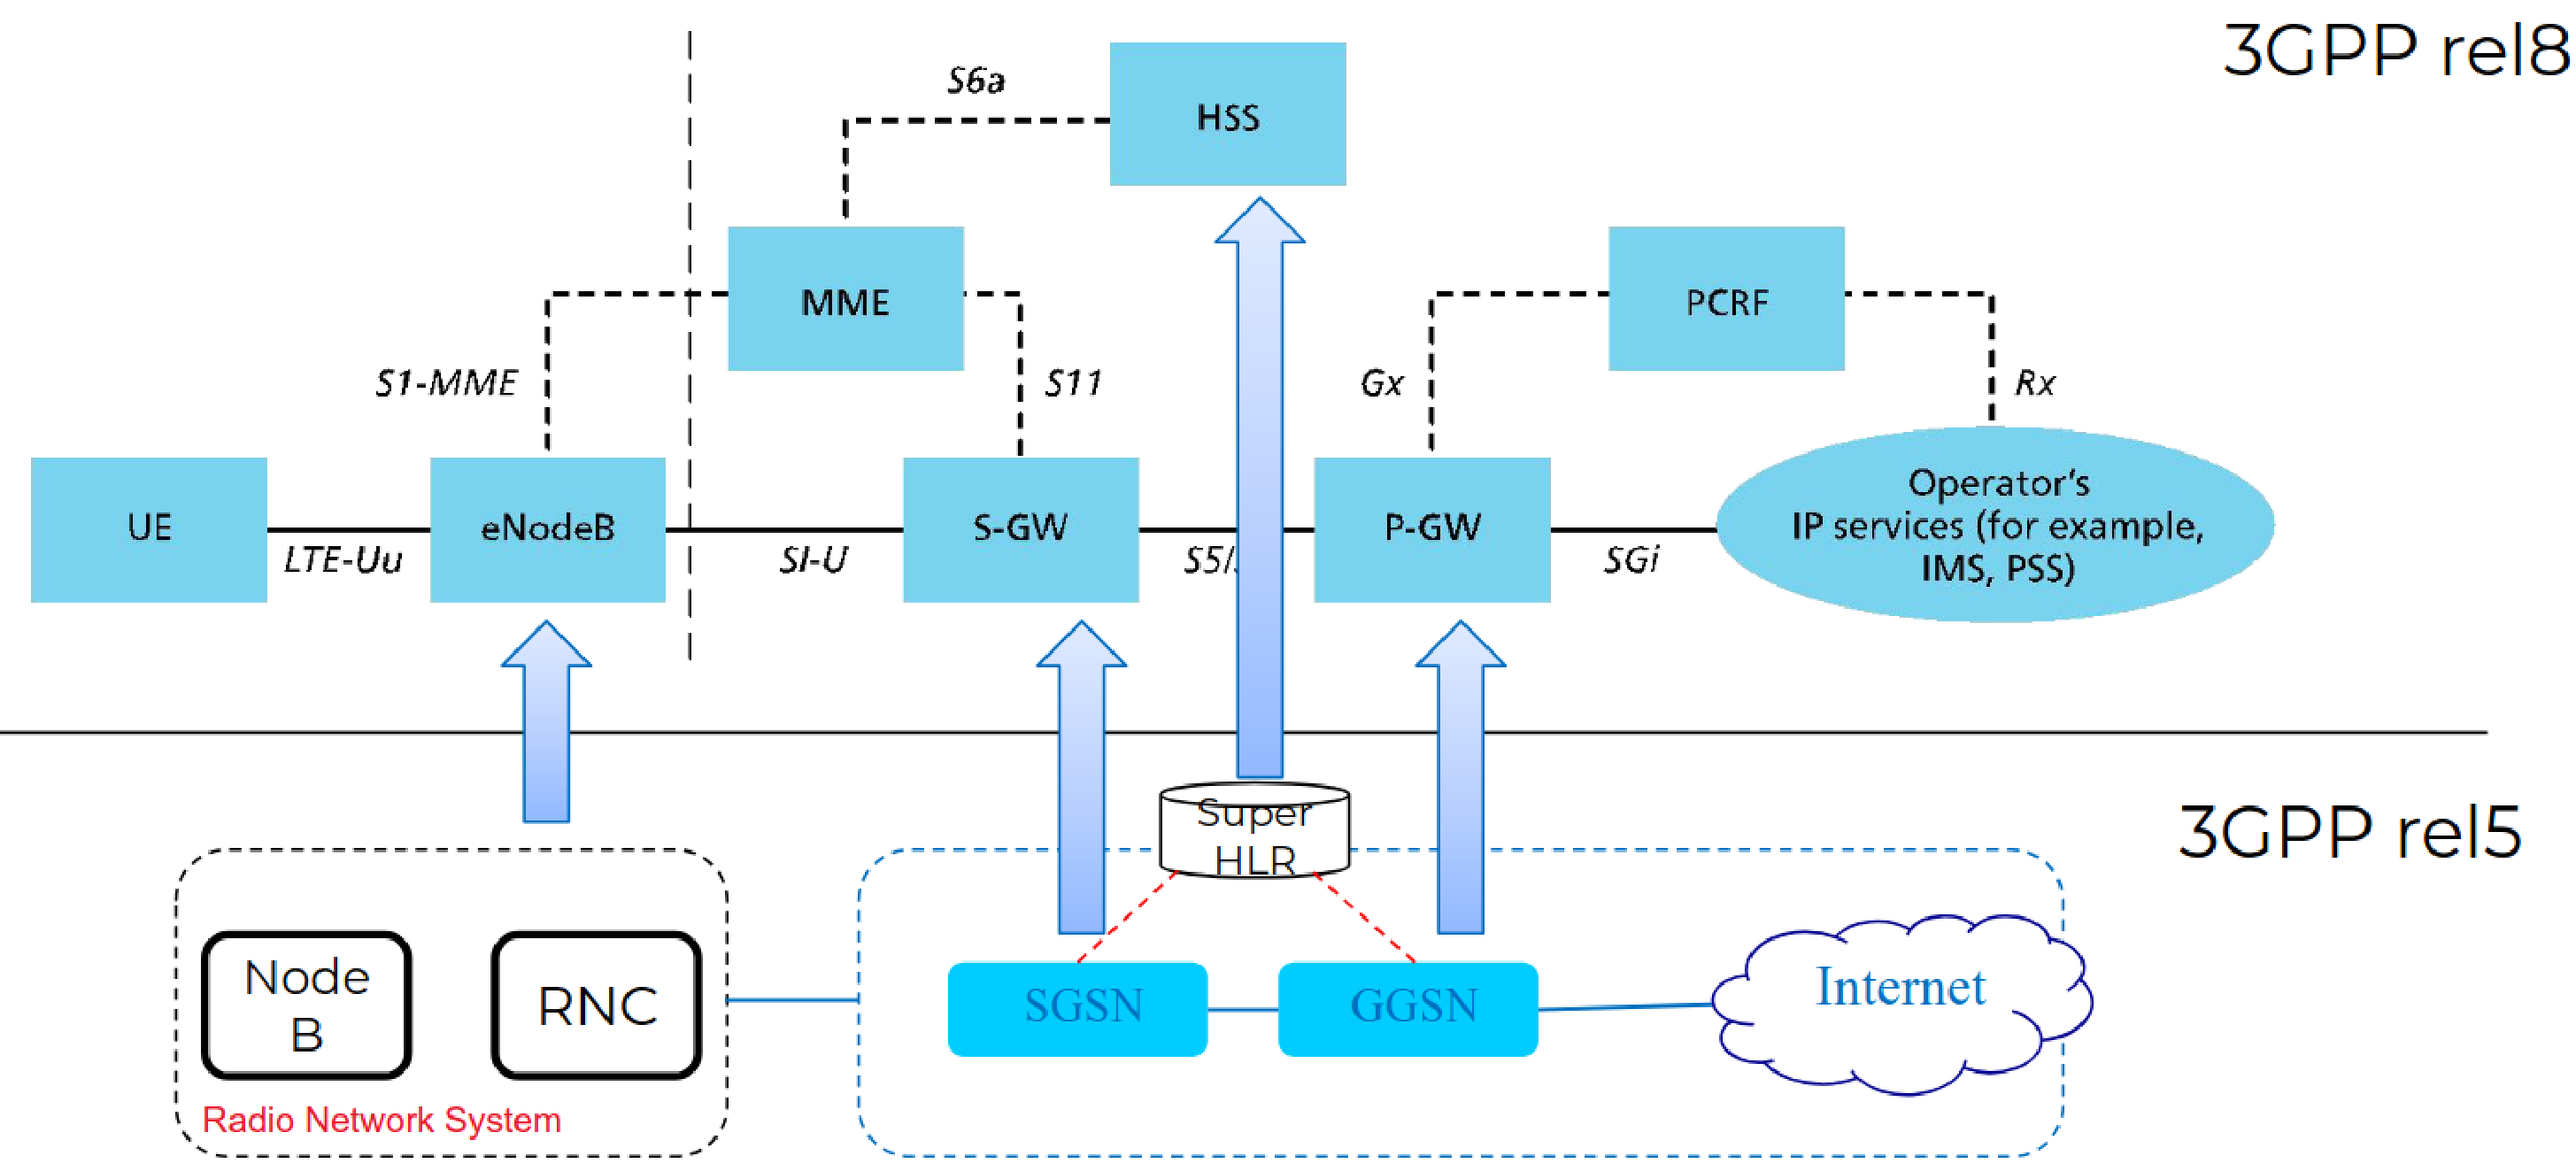
\includegraphics[width=0.95\linewidth]{img/4g/3g4g}
\end{center}

Alcune differenze: 
\begin{center}
	\begin{tabular}{| m{3.5cm} | m{2cm} | m{2cm} |}
		\hline
		& 3G & 4G \\
		\hline
		Separazione logica di Control e Data plane &  No & Sì \\
		\hline
		Accesso multiplo  &WCDMA & OFDMA \\
		\hline
		Riuso frequenze & 100\% & 100\% flessibile \\
		\hline
		Larghezza banda & $5 MHz$ & $1.4$, $3$, $5$, $10$, $15$, $20 MHz$ \\
		\hline		
		Componenti rete accesso & NodeB e RNC & eNodeB \\
		\hline
		Handover & Soft e Hard & Hard \\
		\hline
		Trasporto & Circuito e Packet Switch & Packet Switch \\
		\hline
		Servizi voce e SMS & Interni alla rete & Esterni alla rete \\
		\hline
	\end{tabular}
\end{center}

Si introduce a livello architetturale una \textbf{separazione più netta} anche a livello logico \textbf{tra data e control plane}. Da NodeB (nome 3G per la Base Station) e RNC (Radio Network Controller, si occupa della gestione risorse radio) si ha solo il \textbf{eNodeB} (e sta per "\textit{evolved}"), questo è anche il motivo per cui l'handover è solo hard, non c'è più una RNC che può gestire multiple connessioni. Il dispositivo utente viene chiamato \textbf{User Equipment UE}.\\

La rete si divide in 
\begin{itemize}
	\item \textbf{E-UTRAN (Evolved Universal Terrestrial Radio Access Network)}, che comprende: 
	\begin{itemize}
		\item User Equipment UE
		\item eNodeB
	\end{itemize}
	\item \textbf{EPC (Evolved Packet Core)}, che contiene i moduli: 
	\begin{itemize}
		\item HSS Home Subscriber Server
		\item MME Mobility Management Entity
		\item P-GW Packet Data Network Gateway
		\item PCRF Policy Control and Charging Rules Function
		\item S-GW Serving Gateway
	\end{itemize}
\end{itemize}

\subsection{Core Network}

\subsubsection{Mobility Management Entity MME} 

Si occupa di tutto ciò che è traffico di controllo e segnalazione all'interno della rete; il nodo di controllo responsabile del traffico di segnalazione tra Core Network (CN) e UE attraverso la suite di protocolli NAS (Non-Access Stratum). Tutto ciò che non è dati utente. Si occupa di: 
\begin{itemize}
	\item Gestione del contesto UE tramite operazioni NAS
	\item Gestione dei bearer (creazione, mantenimento, distruzione, \dots)
	\item Gestione della mobilità all'interno della Tracking Area (TA, insieme di BS)
	\item Gestione del paging
	\item Gestione dei aspetti di sicurezza e cifratura (genera e distribuisce chiavi, \dots)
\end{itemize}
Tra dispositivo utente e MME non transita mai traffico dati, solo controllo.\\

\subsubsection{Home Subscriber Server HSS} 

Nodo che contiene le informazioni dell'utente, come: 
\begin{itemize}
	\item Profili Quality of Service QoS ammessi
	\item Eventuali restrizioni roaming
	\item Informazioni APN (Access Point Name)
	\item Identità dell'MME a cui UE è registrato
\end{itemize}

\subsubsection{Packet Data Network Gateway P-GW} 

Nodo al bordo tra rete LTE e reti esterne come Internet. Gestisce: 
\begin{itemize}
	\item Assegnamento dell'IP all'UE
	\item Garantisce QoS policy autorizzate da PCRF
	\item Filtro dei pacchetti IP downlink in bearer differenti per QoS
	\item Gestione della mobilità tra reti non-3GPP (CDMA-2000 o WiMAX)
\end{itemize}

\subsubsection{Serving Gateway S-GW} 

L'unico vero modulo solo data plane, nodo responsabile della gestione del traffico user-plane. Si occupa di:
\begin{itemize}
	\item Gestione di tutti i pacchetti IP degli utenti circolanti nella rete dell'operatore
	\item Funzioni di ancora mobile la gestione dei bearer quando UE è in fase di handover (dentro la tracking area)
	\item Funzionalità di buffering quando UE è in modalità IDLE-CONNECTED
\end{itemize}
Si tratta del punto di gestione, con un sottogruppo di eNodeB e, di conseguenza, utenti.

\subsubsection{Policy Control and Charging Rules Function PCRF} 

Svolge le funzioni di 
\begin{itemize}
	\item Controllo e autorizzazioni per singolo flusso a livello di P-GW
	\item Autorizza QoS secondo il profilo dell'utente (da HSS)
\end{itemize}
Contiene le "regole" da applicare all'utente, da negoziare e far applicare dal P-GW.

\subsubsection{Servizi operatore} 

I servizi sono esterni alla rete: 
\begin{itemize}
	\item Chiamate: Voice over LTE (VoLTE): VoIP su rete LTE
	\item Internet
\end{itemize}

\hfill \\

\subsection{E-UTRAN}

\subsubsection{Evolved-NodeB eNodeB} 

Primo all'interno di E-UTRAN; fornisce connettività radio all'UE e lo collega alla Core Network. Ha i compiti di una BS:
\begin{itemize}
	\item Gestione delle risorse radio
	\item Gestione dell'accesso multiplo di più UE
	\item Compressione degli header (utile per traffico VoIP)
	\item Connessione con S-GW e MME per traffico dati e controllo
	\item Informazioni sulla posizione degli UE
	\item Sicurezza e crittografia del canale radio
\end{itemize}
Prima di questo era tutto cablato, questa è la prima parte wireless.\\

\subsubsection{Modulazione e Codifica Trasmissione}

Non verrà considerato, il Multiple Access, singolo utente. Con QPSK. Si ha una codifica digitale da tradurre in onde radio, a partire dai bit il processo di \textbf{trasmissione} è:
\begin{itemize}
	\item codifica dei bit in simboli tramite QPSK, 2 bit per simbolo
	\item modulazione usando una frequenza intermedia (IF); in LTE questa frequenza permette di variare leggermente la frequenza della portante (es: OFDMA lo usa per gestire più utenti)
	\item conversione in analogico (DAC)
	\item modulazione sulla portante: da banda base a banda traslata sulla portante
	\item selezione della componente in fase 
	\item trasmissione
\end{itemize}
\begin{center}
	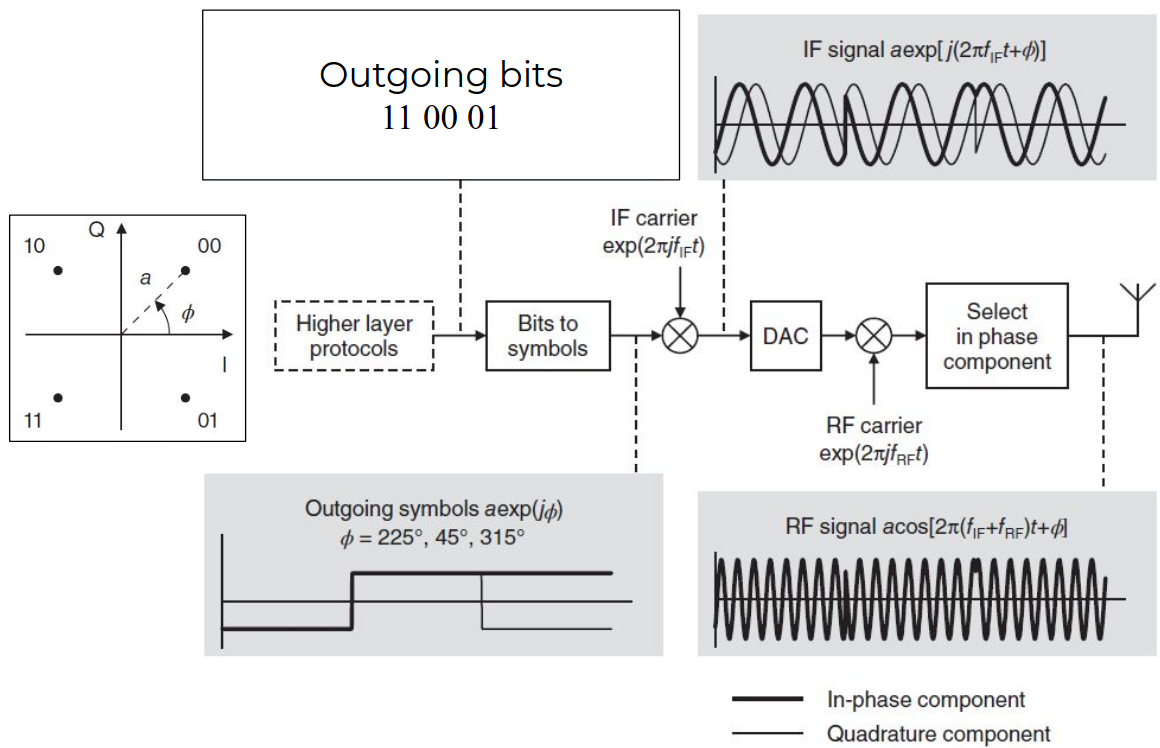
\includegraphics[width=0.9\linewidth]{img/4g/mightbesending}
\end{center}

In \textbf{ricezione}: 
\begin{itemize}
	\item si misura sull'antenna il segnale, con relativo rumore e sfasamento indotto dalla mobilità ($\psi$)
	\item rimuovo la frequenza portante, torno in banda base
	\item filtro passa-basso per eliminare il rumore termico
	\item convertitore analogico digitale (ADC)
	\item Abbiamo trasmesso $\varphi$ e ricevuto $\varphi + \psi$ (sfasatura), per capire quanto è sfasato si fa channel estimation: stima dello sfasamento dovuto al canale (condizioni del canale), fatto tramite la ricezione di un pilot standard, per poi togliere quello sfasamento dall'onda dati ricevuta
	\item conversione da simboli a bit
\end{itemize}

\newpage

Le \textbf{codifiche possibili} sono:
\begin{itemize}
	\item \textbf{BPSK Binary Phase Shift Keying}: usato solo per alcuni segnali di controllo a basso livello; non importa la qualità del canale, alcuni segnali di controllo fondamentali devono essere "compresi"
	\item \textbf{QPSK Quadrature Phase Shift Keying}: usato per tutti i messaggi radio di controllo e trasmissione dati in caso di scarsa qualità del segnale; permette un minore overhead di controllo, mantenendo una buona "comprensibilità" del segnale
	\item \textbf{16/64-QAM Quadrature Amplitude Modulation}: usato per la trasmissione dati
\end{itemize}

\paragraph{Scelta di modulazione e codifica:} Si ha un Adapting Modulation e Coding scheme: quantifica la qualità del canale in 4 bit e sceglie una modulazione:
\begin{center}
	\begin{tabular}{>{\centering\arraybackslash}m{0.8cm} >{\centering\arraybackslash}m{3cm} >{\centering\arraybackslash}m{3.5cm} >{\centering\arraybackslash}m{3.5cm}}
		\toprule
		\textbf{CQI} & \textbf{Modulation scheme} & \textbf{Coding rate (units of 1/1024)} & \textbf{Information bits per symbol} \\
		\midrule
		0  & n/a     & 0   & 0.00 \\
		1  & QPSK    & 78  & 0.15 \\
		2  & QPSK    & 120 & 0.23 \\
		3  & QPSK    & 193 & 0.38 \\
		4  & QPSK    & 308 & 0.60 \\
		5  & QPSK    & 449 & 0.88 \\
		6  & QPSK    & 602 & 1.18 \\
		7  & 16-QAM  & 378 & 1.48 \\
		8  & 16-QAM  & 490 & 1.91 \\
		9  & 16-QAM  & 616 & 2.41 \\
		10 & 64-QAM  & 466 & 2.73 \\
		11 & 64-QAM  & 567 & 3.32 \\
		12 & 64-QAM  & 666 & 3.90 \\
		13 & 64-QAM  & 772 & 4.52 \\
		14 & 64-QAM  & 873 & 5.12 \\
		15 & 64-QAM  & 948 & 5.55 \\
		\bottomrule
	\end{tabular}
\end{center}

Esempio: con CQI 7 si hanno 1.48 bit di informazione per ogni simbolo, quindi per 1024 bit 378 saaranno di informazione. Queste valgono per il data plane, il control plane ha una sua codifica molto meno variabile.\\

\subsubsection{Riuso frequenze}
\begin{center}
	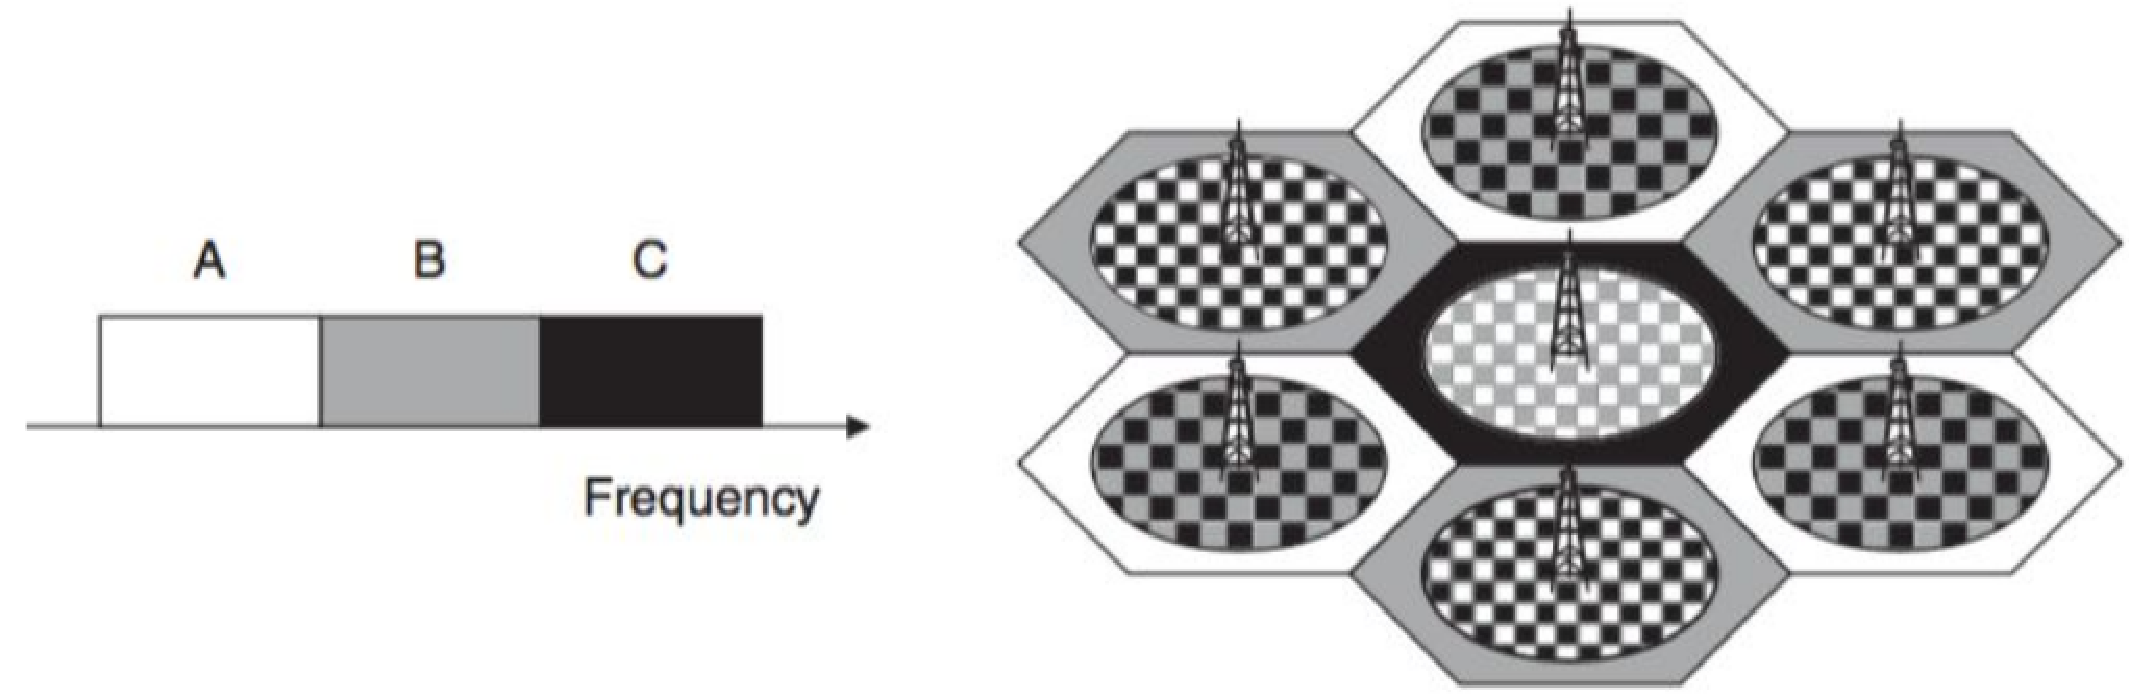
\includegraphics[width=0.9\linewidth]{img/4g/riuso4g}
\end{center}
Utilizzo del 100\% delle frequenze disponibili come in UMTS.  Rispetto a UMTS la gestione delle interferenze è più semplice e coordinata tra le celle tramite l’apposita interfaccia X2. Le frequenze vengono coordinate ai bordi delle celle, in modo da usare una banda maggiore al centro, dove non possono esserci interferenze.\\

\subsubsection{Durata Simboli}

Non è casuale, si è decisa in base a
\begin{itemize}
	\item la distanza tra sottoportanti $15kHz$
	\item punti da campionare per la trasformata di Fourier $2048$
\end{itemize}

Di conseguenza
$$ T_S = \frac{1}{2048 \cdot 15000}s \approx 32.6 ns $$

Quindi il processore fisico deve avere una velocità adeguata. Un simbolo dura $2048 T_S = 66.7 \mu s$.\\

\newpage

\subsubsection{Struttura Slot}
I simboli sono organizzati in slot da $0.5ms$ ($15360 T_S$).\\

Si ha un cyclic prefix per evitare interferenza inter-simbolo causa del multipath. Per ogni slot ci sono 7 simboli ($66.7 \mu s$ ognuno), di cui $4.7$ o $5.2 \mu s$ sono di preambolo.
\begin{center}
	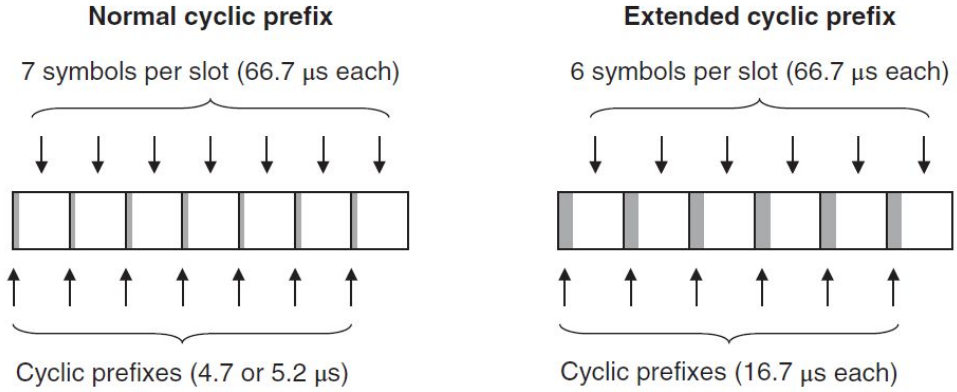
\includegraphics[width=0.7\linewidth]{img/4g/cycprefix}
\end{center}

\subsubsection{Duplex}

Per la gestione del duplex, ogni eNodeB può essere configurato in 2 modalità comunicate a UE durante la fase di configurazione: 
\begin{itemize}
	\item \textbf{Frequency Division Duplex (FDD)}: Utilizzo di frequenze diverse per uplink e downlink
	\begin{center}
		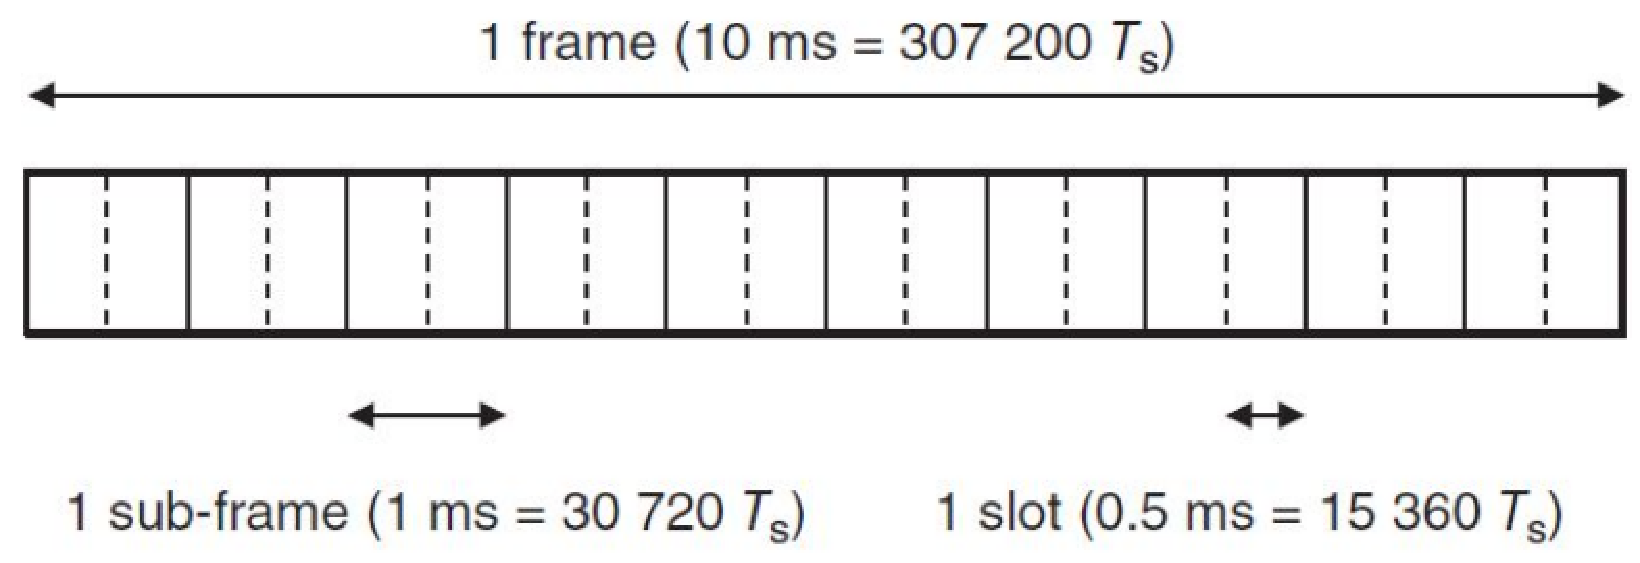
\includegraphics[width=0.5\linewidth]{img/4g/fdd}
	\end{center}
	ogni frame di $10ms = 307200 T_S$ contiene 10 subframe/20 slot da $1/0.5ms$, quindi si hanno 140 simboli/frame (20x7) con normal cyclic prefix e 120 simboli/frame (20x6) con extended cyclic prefix.\\
	
	\item \textbf{Time Division Duplex (TDD)}: Utilizzo di una sola frequenza per uplink e downlink. Sono possibili 7 configurazioni:
	\begin{center}
		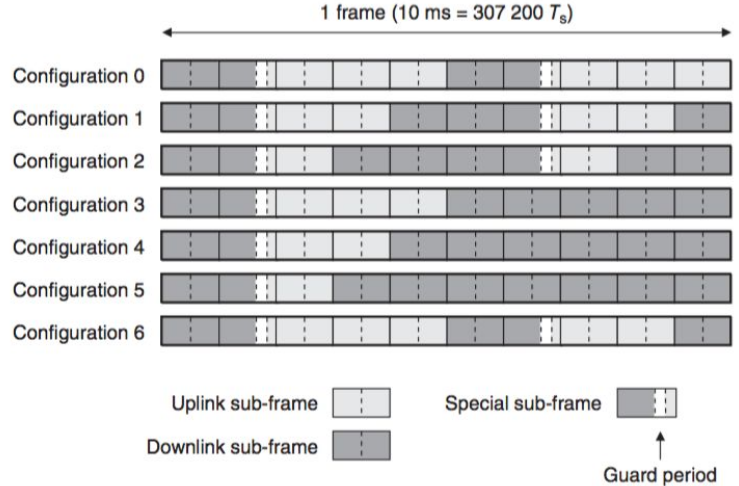
\includegraphics[width=0.7\linewidth]{img/4g/tdd}
	\end{center}
	La configurazione è decisa in base all'utilizzo (se serve più downlink ne metto di più e viceversa).
\end{itemize}

\paragraph{Uplink Timing Advance:} Il guard period tiene conto dell'anticipo di trasmissione in uplink (Uplink Timing Advance). UE inizia a trasmettere in uplink in anticipo rispetto al tempo del frame della base station, altrimenti la ricezione avverrebbe in maniera disallineata dal tempo degli slot della BS, dato che dispositivi più lontani ci mettono più tempo a far arrivare il segnale. \\

Viene fornito un range di timing advance tra $0$ e $667\mu s$ per compensare la distanza. Per fare questo serve però che nessuno stia parlando in downlink durante il tempo di advance (altrimenti si avrebbe interferenza), per questo il guard time: serve a permettere l'advance per l'uplink senza interferenze.\\

\newpage

\subsubsection{Orthogonal Frequency Division Multiple Access OFDMA}

Gli eNodeB usano OFDMA: la banda viene divisa in piccole sotto-bande (sub-carriers) le cui frequenze non causano interferenze. LTE usa sotto-bande di ampiezza $15 kHz$ (frequenze intermedie IF di modulazione ortogonali). Più sotto-bande sono organizzate in \textbf{Resource Block} che rappresentano la minima quantità di risorse allocabili ad un singolo dispositivo.

\begin{center}
	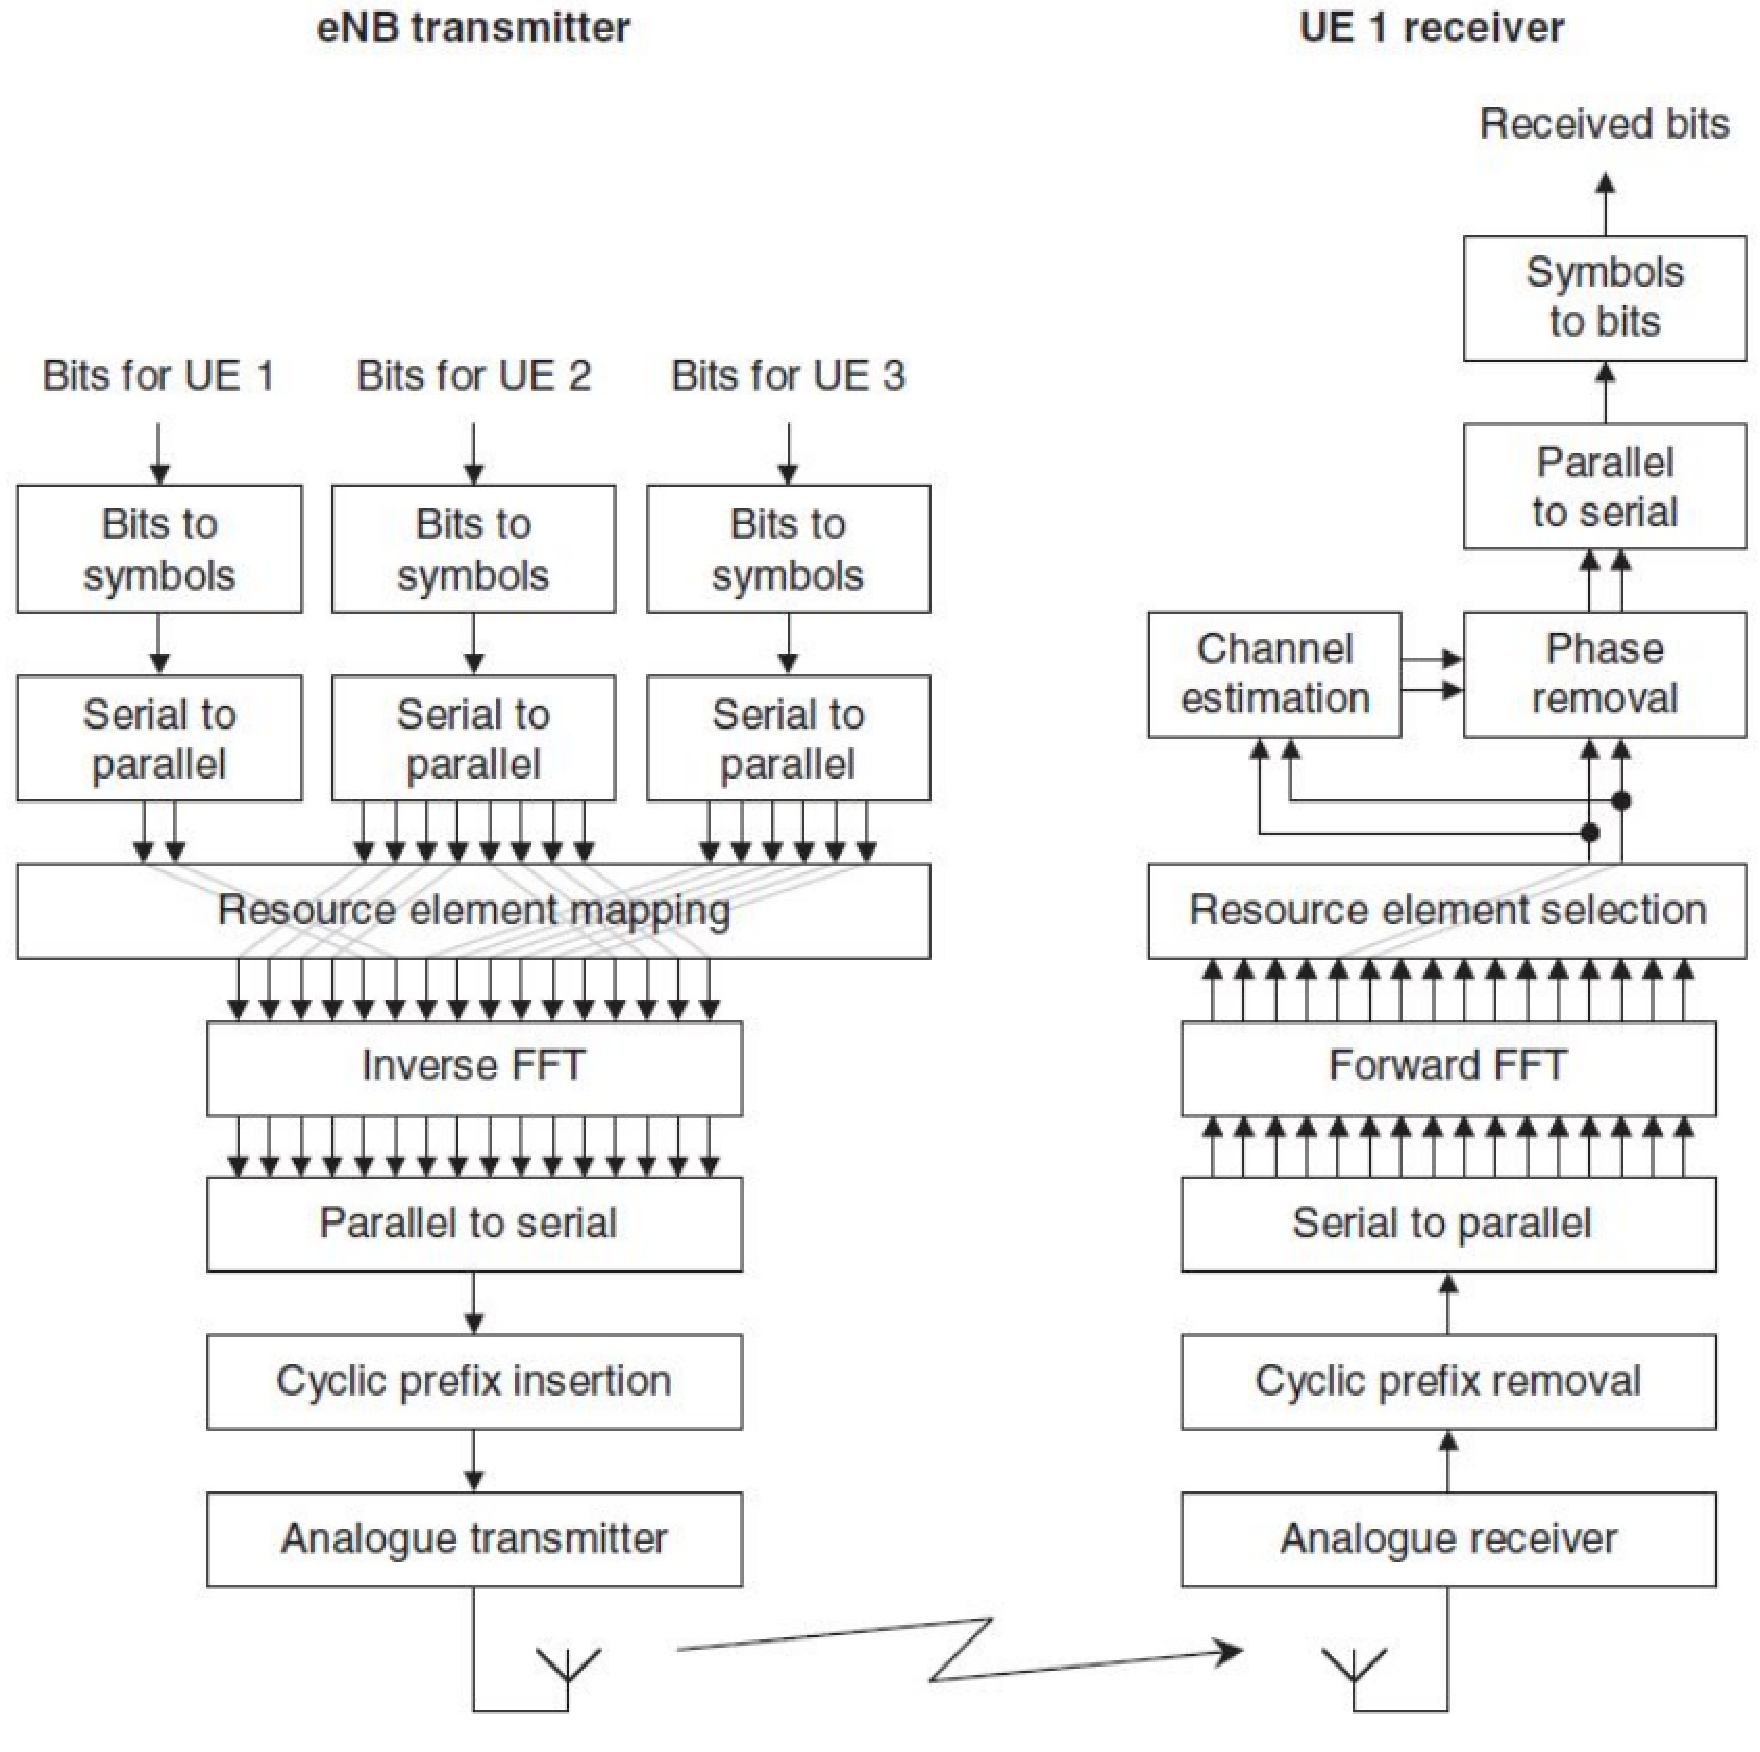
\includegraphics[width=0.75\linewidth]{img/4g/utranofdma}
\end{center}

Gli step lato trasmettitore sono: 
\begin{itemize}
	\item Ogni flusso di bit distinto viene trasformato in simboli
	\item I simboli vengono mappati sulle risorse in frequenza (resource block allocati)
	\item Si applica la IFFT per trasformare i simboli mappati in frequenza nel dominio del tempo, ottenendo il segnale OFDM complesso
	\item I campioni temporali paralleli vengono ricombinati in un unico flusso seriale
	\item Si aggiunge il prefisso ciclico
	\item Il segnale viene convertito in analogico e trasmesso
\end{itemize}
Lato ricevitore bisogna fare il processo contrario, estraendo il flusso di bit per l'UE che sta ricevendo (sceglie di considerare solo i resource block a lui dedicati), correggendo il flusso dal rumore e sfasamento (tramite channel estimation).\\

Si hanno 12 sotto-bande di larghezza minima $180 kHz$ e 7 simboli in $0.5ms$. \\

\subsubsection{eNodeB Scheduler}
Tutte le comunicazioni da e per i dispositivi sono gestite dall'eNodeB. Lo scheduling ha risorse a disposizione (resource blocks) e determina come allocarli
\begin{center}
	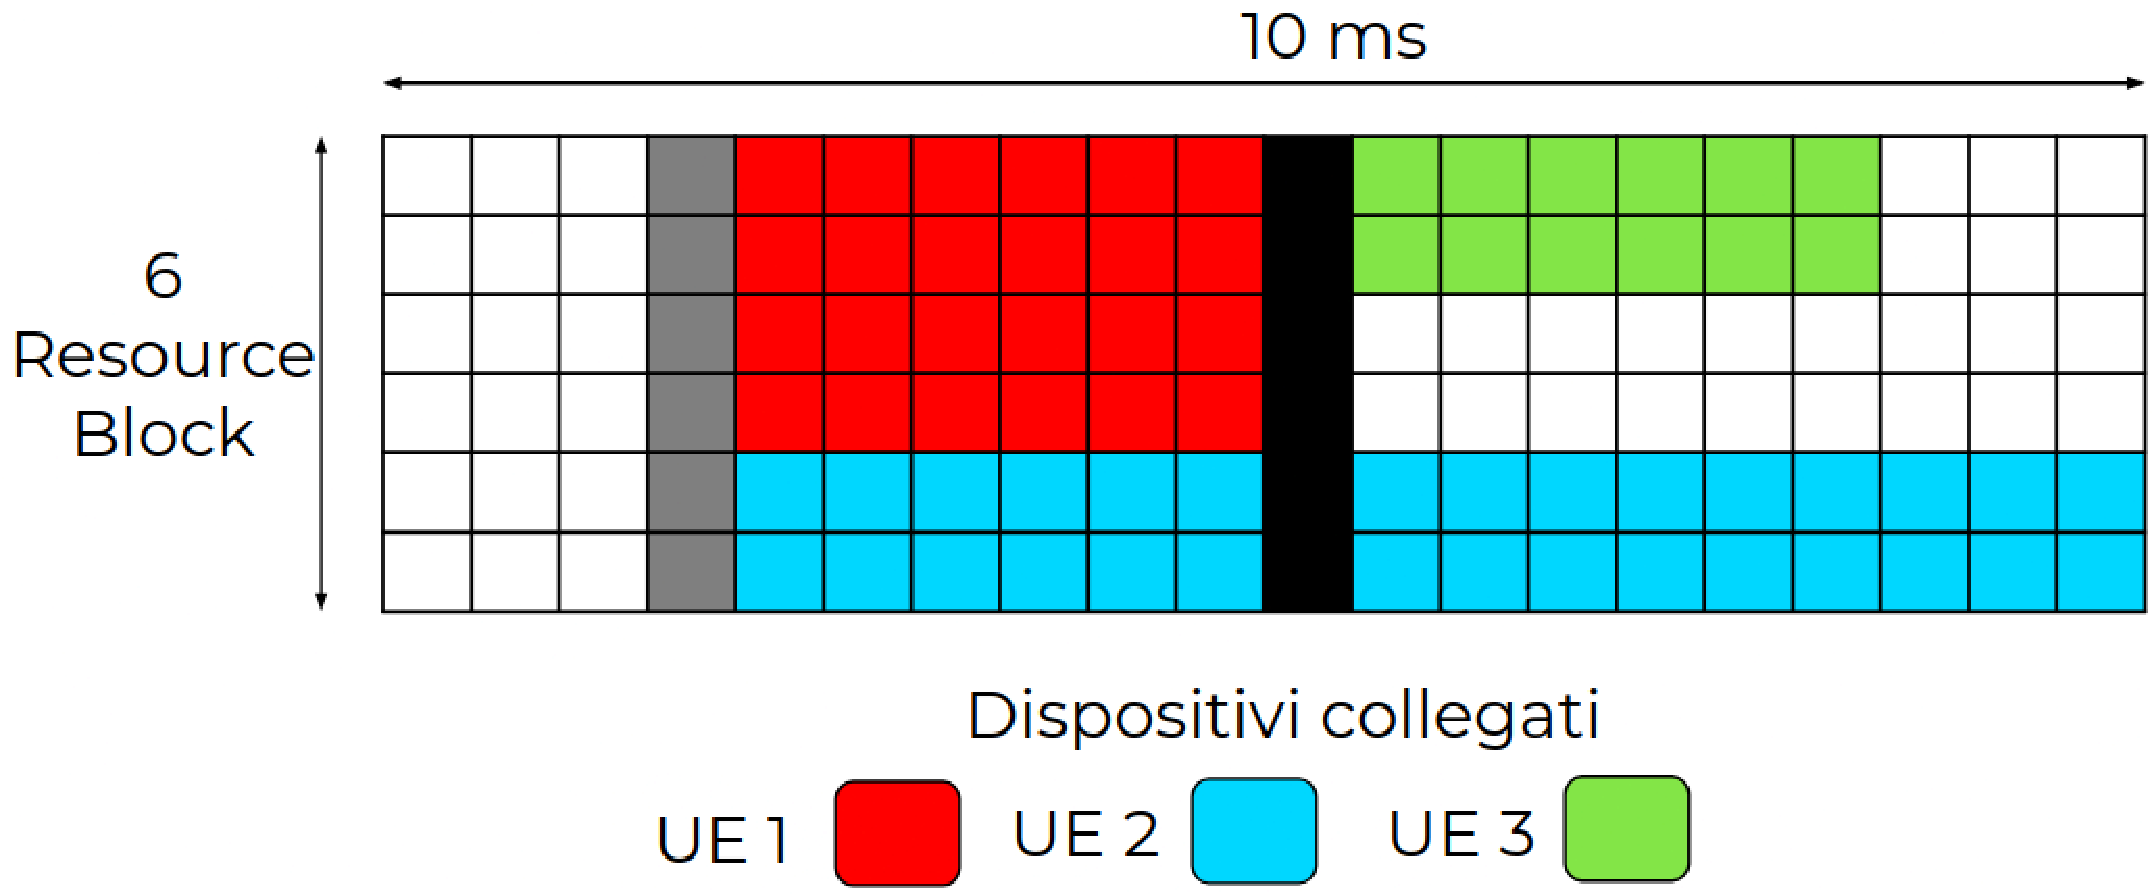
\includegraphics[width=0.75\linewidth]{img/4g/alloc}
\end{center}
Blocchi grigi e neri sono dedicati alla trasmissione della BS. Tutto lo scheduling deve essere fatto real time (i.e., molto veloce).\\

\subsubsection{Velocità per UE}

Alla fine la banda disponibile per ogni singolo dispositivo dipende da molti fattori: 
\begin{itemize}
	\item Capacità del dispositivo (UE)
	\item Qualità del segnale radio: interferenze e distanza, determina la scelta della codifica
	\item Larghezza della banda in MHz: maggiore banda, maggior numero di resource block allocabili
	\item Configurazione TDD: a seconda della configurazione dell'eNodeB si possono avere differenti velocità di upload e download
	\item Numero dispositivi collegati
	\item Altri fattori non dipendenti dal canale radio: come congestione rete backhaul, congestione P-GW o altri fattori end-to-end
\end{itemize}

Le massime velocità teoriche per LTE Rel8 sono $300Mbps$ in download e $75Mbps$ in upload.\\

%End L17

\subsubsection{Collegamento alla Core Network}

Si aggiunge un collegamento diretto tra BS, tramite un'interfaccia denominata X2, con una suite di protocolli dedicata. Questo permette di svolgere compiti locali tra le BS.\\

Schema logico e fisico:
\begin{center}
	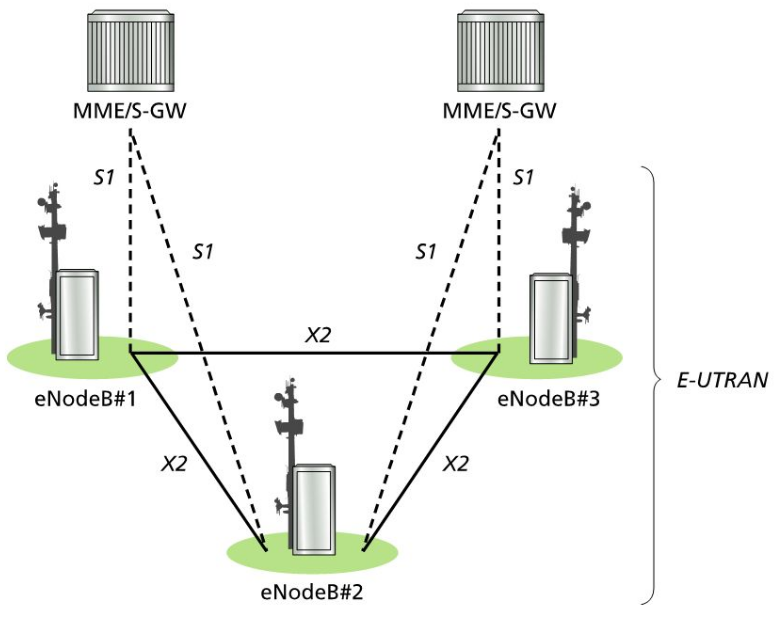
\includegraphics[width=0.6\linewidth]{img/4g/x21}
\end{center}

\newpage

\subsubsection{Tracking Area}

Per questioni di fault tolerance, ridondanza e load balancing si ha un \textbf{raggruppamento delle BS in Tracking Areas TAs}. Visto come un cluster di BS. A ciascuno di questi cluster sono associati uno o più gruppi di moduli di controllo.
\begin{center}
	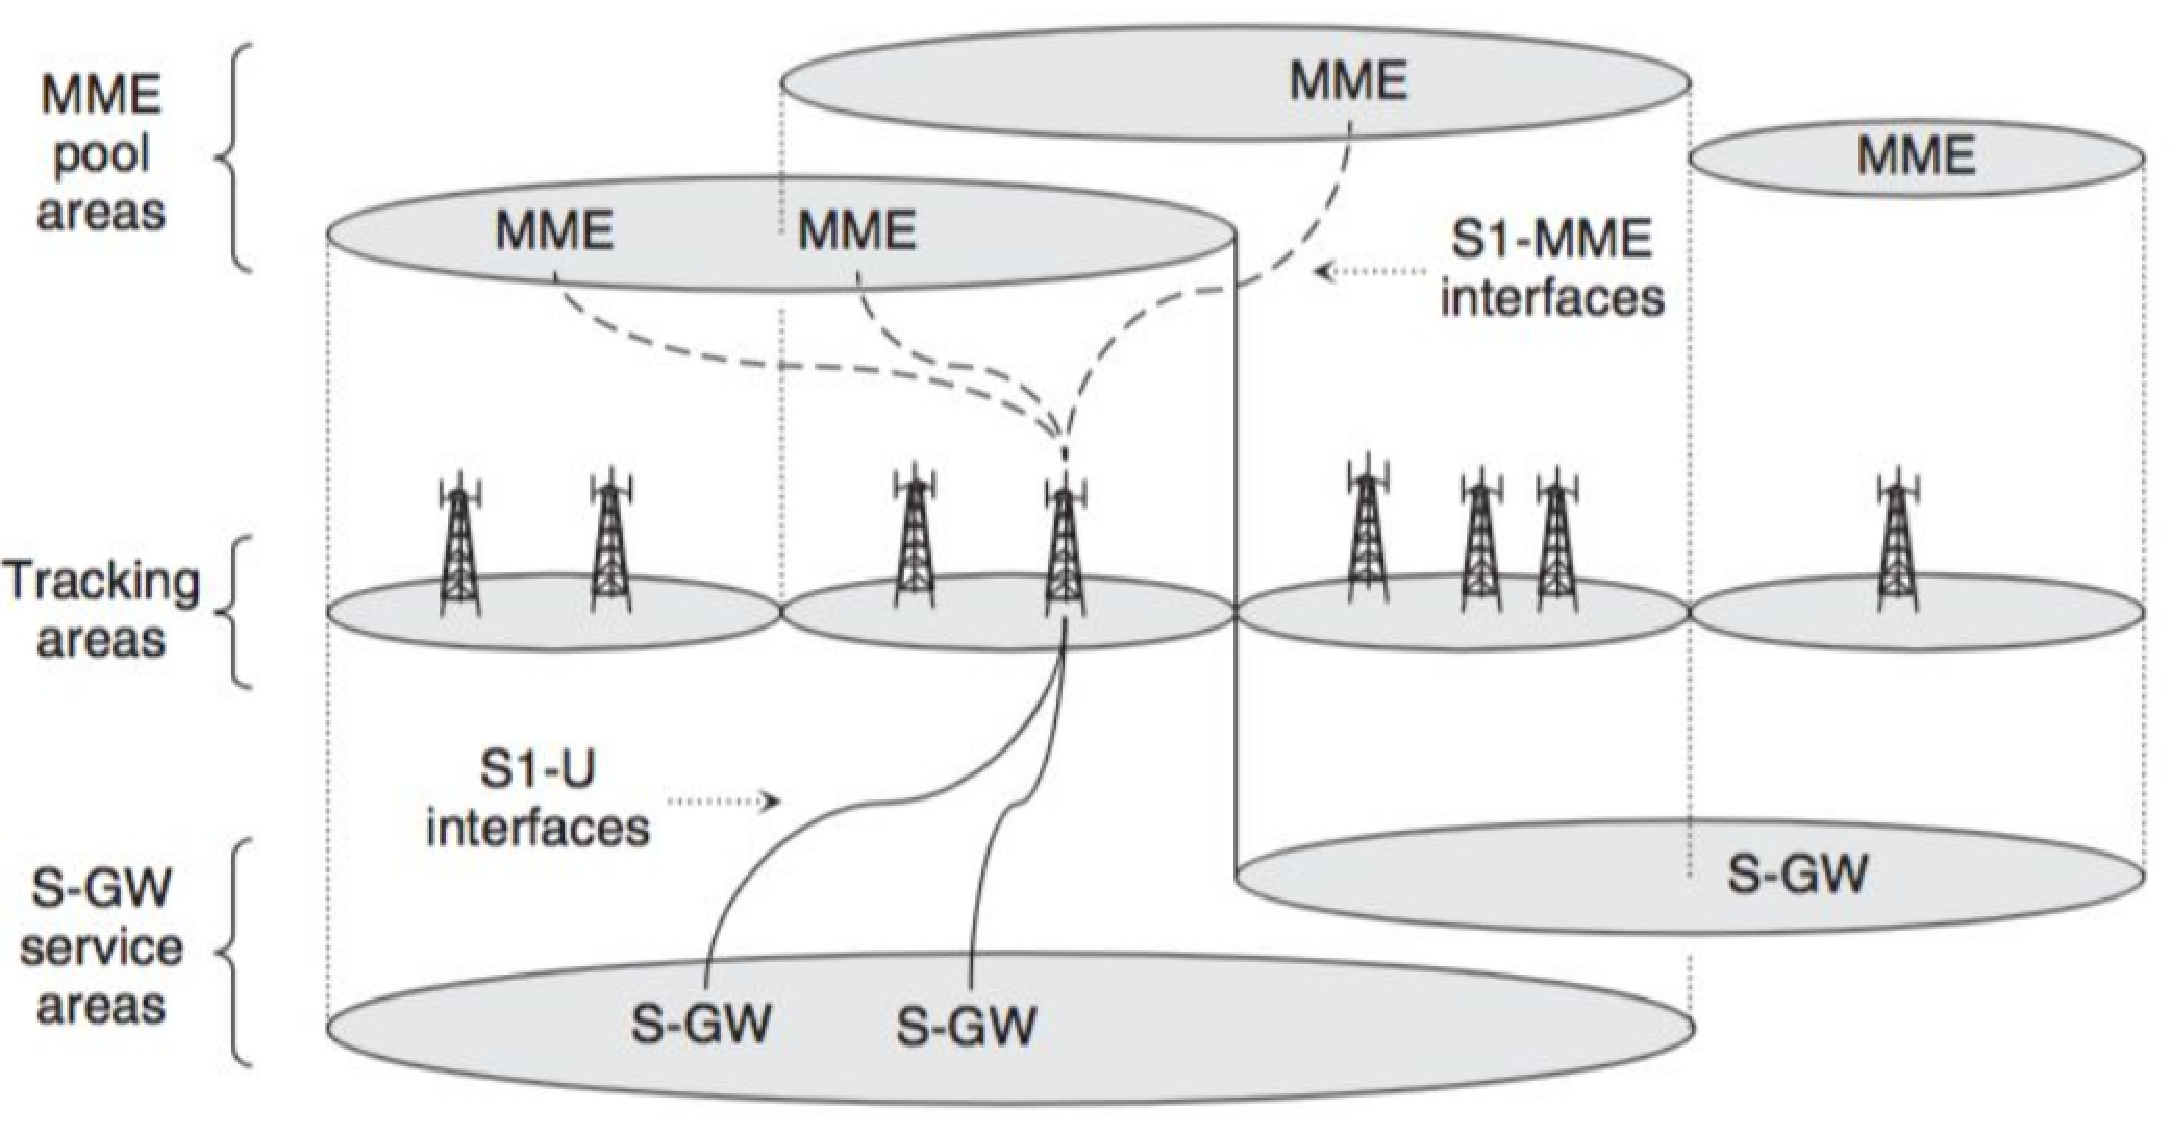
\includegraphics[width=0.7\linewidth]{img/4g/tas}
\end{center}

\subsubsection{Interfaccia X2}

La suite di protocolli dell'interfaccia X2 permette la \textbf{comunicazione diretta tra eNodeB}. Permette: 
\begin{itemize}
	\item gestione handover in alternativa a S1
	\item funzionalità Self-Organizing Network (SON): load balancing, gestione delle interferenze
	\item mantenimento dello storico delle ultime celle visitate per gestire l'effetto Ping-Pong tra celle
\end{itemize}

In generale, oltre ad essere un canale di handover alternativo, permette meccanismi SON, coordinazione radio, load balancing dinamico e altre funzionalità per migliorare l'efficienza della rete.\\

\newpage

\subsection{Architettura}

\subsubsection{Control Plane}

Si ha una netta separazione tra control e data plane. I moduli direttamente coinvolti nel control plane sono UE, eNodeB e MME.\\

Lo \textbf{stack} di protocolli è:
\begin{center}
	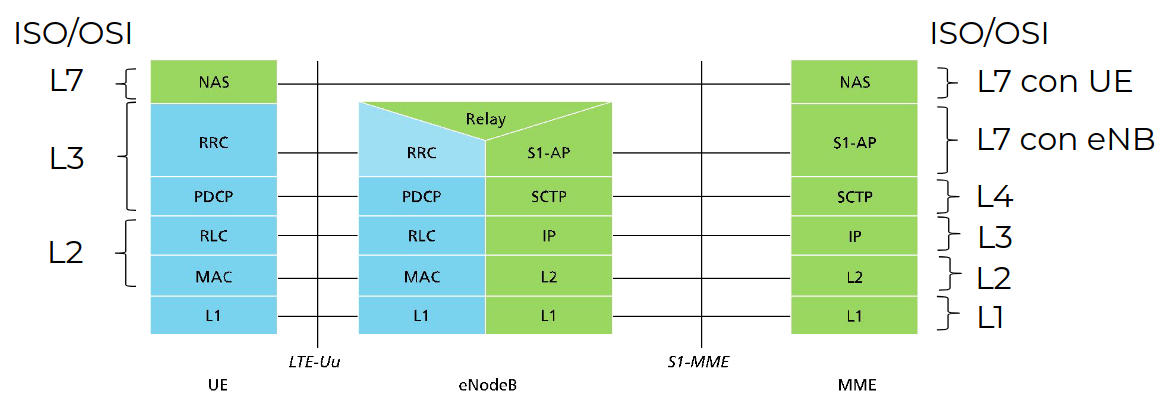
\includegraphics[width=0.9\linewidth]{img/4g/cps}
\end{center}

A lato indicato l'equivalente ISO/OSI. La BS è dual stack in quanto deve parlare con entrambi i lati. Livello 1 e 2 non sono specificati in quanto "a scelta".\\

\paragraph{UE - eNodeB:} A sinistra c'è la parte di UE, i protocolli (dall'alto verso il basso) sono:
\begin{itemize}
	\item \textbf{Radio Resource Control RRC}:
	\begin{itemize}
		\item gestisce il paging, le informazioni di paging passano per questo livello
		\item gestisce la mobilità, viene deciso l'handover
		\item si occupa di QoS e raccolta misurazioni UE
	\end{itemize}
	
	\item \textbf{Packet Data Convergence Protocol PDCP}:
	\begin{itemize}
		\item convergenza tra mondo IP e mobile, comprime gli header, mandando di fatto solo le differenze
	\end{itemize}
	
	\item \textbf{Radio Link Control RLC}:
	\begin{itemize}
		\item correzione errori
		\item gestione ritrasmissione
		\item segmentazione/riassemblaggio dei pacchetti dei livelli superiori
	\end{itemize}
	
	\item \textbf{Medium Access Control MAC}:
	\begin{itemize}
		\item gestione dell'accesso al canale radio
		\item gestione dello scheduler (da eNodeB)
	\end{itemize}
\end{itemize}

\paragraph{eNodeB - MME:} L'altro lato include: 
\begin{itemize}
	\item \textbf{Livello applicazione interfaccia S1 S1-AP}:
	\begin{itemize}
		\item trasporto di tutto il traffico di controllo tra E-UTRAN e Core Network
	\end{itemize}
	
	\item Stream Control Transmission Protocol SCTP: 
	\begin{itemize}
		\item protocollo di livello trasporto utilizzato per ottimizzare il trasporto del traffico di segnalazione
	\end{itemize}
	
	\item \textbf{Internet Protocol IP} (interna alla rete operatore):
	\begin{itemize}
		\item eNB: indirizzo IP interno alla rete operatore per identificare uno specifico eNB nella rete
		\item MME: indirizzo IP interno alla rete che identifica uno specifico MME nella rete
		\item Il routing dei messaggi control plane
	\end{itemize}
\end{itemize}

\paragraph{SCTP - Motivazioni:} Le motivazioni dietro SCTP sono:
\begin{enumerate}
	\item TCP fornisce solo trasporto affidabile e in ordine: la consegna è solo affidabile e non permette ordine parziale
	\item Head of Line Blocking Problem
	\item TCP è stream oriented, le applicazioni aggiungono marker specifici per delimitare i messaggi
	\item Supporto Multi-Homing mancante: le connessioni sono esclusivamente da e verso una singola entità
\end{enumerate}

\newpage

\paragraph{Head of Line HOL Block Problem:} In TCP tutto deve essere \textit{in ordine}, ogni cosa ricevuta  può essere passata al livello superiore se e solo se il segmento è in ordine rispetto agli altri. Se viene perso un segmento, i pezzi successivi sono bufferati ma non possono essere passati al livello applicativo perché manca un segmento precedente.\\

Applicato al collegamento eNodeB-MME vorrebbe dire avere un flusso unico per i dati di tutti i dispositivi collegati alla BS. 
\begin{center}
	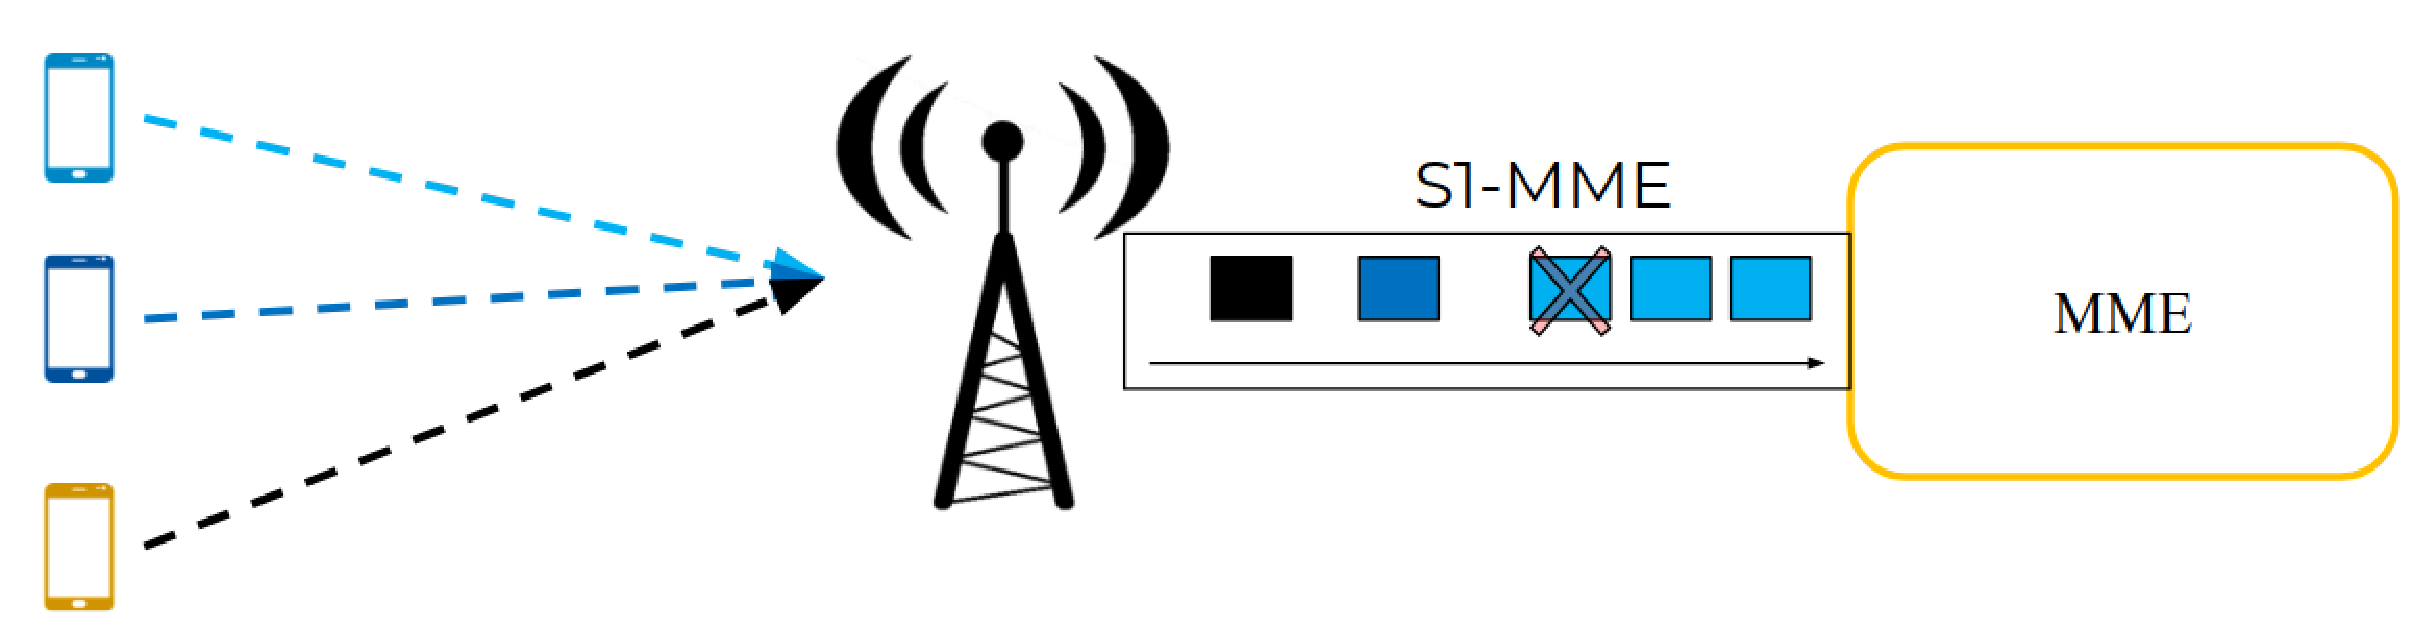
\includegraphics[width=0.7\linewidth]{img/4g/holprob1}
\end{center}

Tutti i pacchetti fanno parte di un cumulative ack, la perdita di un pacchetto vorrebbe dire bloccare tutti gli altri. Non rende indipendenti i dispositivi tra loro.\\

Una prima soluzione potrebbe essere aprire connessioni separate per ogni dispositivo gestito dall'eNodeB: questa non è una soluzione abbastanza scalabile e utilizza troppe risorse (dell'MME principalmente, una porta per dispositivo su tutte le BS che gestisce è decisamente troppo).\\

La \textit{vera} soluzione è usare SCTP: viene aggiunto uno \textbf{stream ID} (16 bit) ai pacchetti, definendo \textbf{multipli stream} all'interno di una \textbf{singola connessione}. Se si perde un pacchetto, vengono bloccati solo i pacchetti con lo stesso stream ID, non gli altri. Una singola connessione ha al suo interno più stream indipendenti, ognuno dei quali ha dati completamente separati. Orientato alla connessione e affidabile, garantisce che i pacchetti arrivino a destinazione in ordine (anche parziale, ordine dello stream, non sulla connessione totale).\\

\newpage

SCTP permette anche il \textbf{Multi-Homing}: non viene usata la quadrupla tipica di TCP, ma l'identificazione della connessione viene fatta tramite gruppi di indirizzi sorgente e destinazione. Identificatori: 
\begin{center}
	\begin{tabular}{l l}
		TCP & <SRC Address, SRC Port, DST Address, DST Port> \\
		SCTP & < \textbf{\{SRC Addresses\}}, SRC port, \textbf{\{DST Addresses\}}, DST port>
	\end{tabular}
\end{center}

TCP aggiunge delimitatori e richiede parsing dei messaggi a livello di applicazione, è stream oriented. SCTP invece è Message Oriented (come UDP), divide i singoli messaggi, si occupa di gestire frammentazione, gestione di flusso e di errori.\\

\paragraph{Confronto SCTP-TCP-UDP:}
\begin{center}
	\begin{tabular}{lccc}
		\toprule
		\textbf{Feature} & \textbf{SCTP} & \textbf{TCP} & \textbf{UDP} \\
		\midrule
		Message‐Oriented                              & X &   & X \\
		Byte‐Oriented                                 &   & X &   \\
		Connection‐Oriented                           & X & X &   \\
		Full‐Duplex                                   & X & X & X \\
		Trasporto affidabile                          & X & X &   \\
		Consegna in ordine                            & X & X &   \\
		Consegna NON in ordine               & X &   & X \\
		Controllo di flusso e di congestione          & X & X &   \\
		ECN (Explicit Congestion Notification)        & X &   &   \\
		Multi‐Streaming                               & X &   &   \\
		Multi‐Homing                                  & X &   &   \\
		Prevenzione SYN flooding attack               & X &   &   \\
		\bottomrule
	\end{tabular}
\end{center}

\newpage

\subsubsection{User Plane}

I moduli coinvolti nell'user plane sono: UE, eNodeB, S-GW, P-GW, servizi operatore.\\

Lo \textbf{stack} è 
\begin{center}
	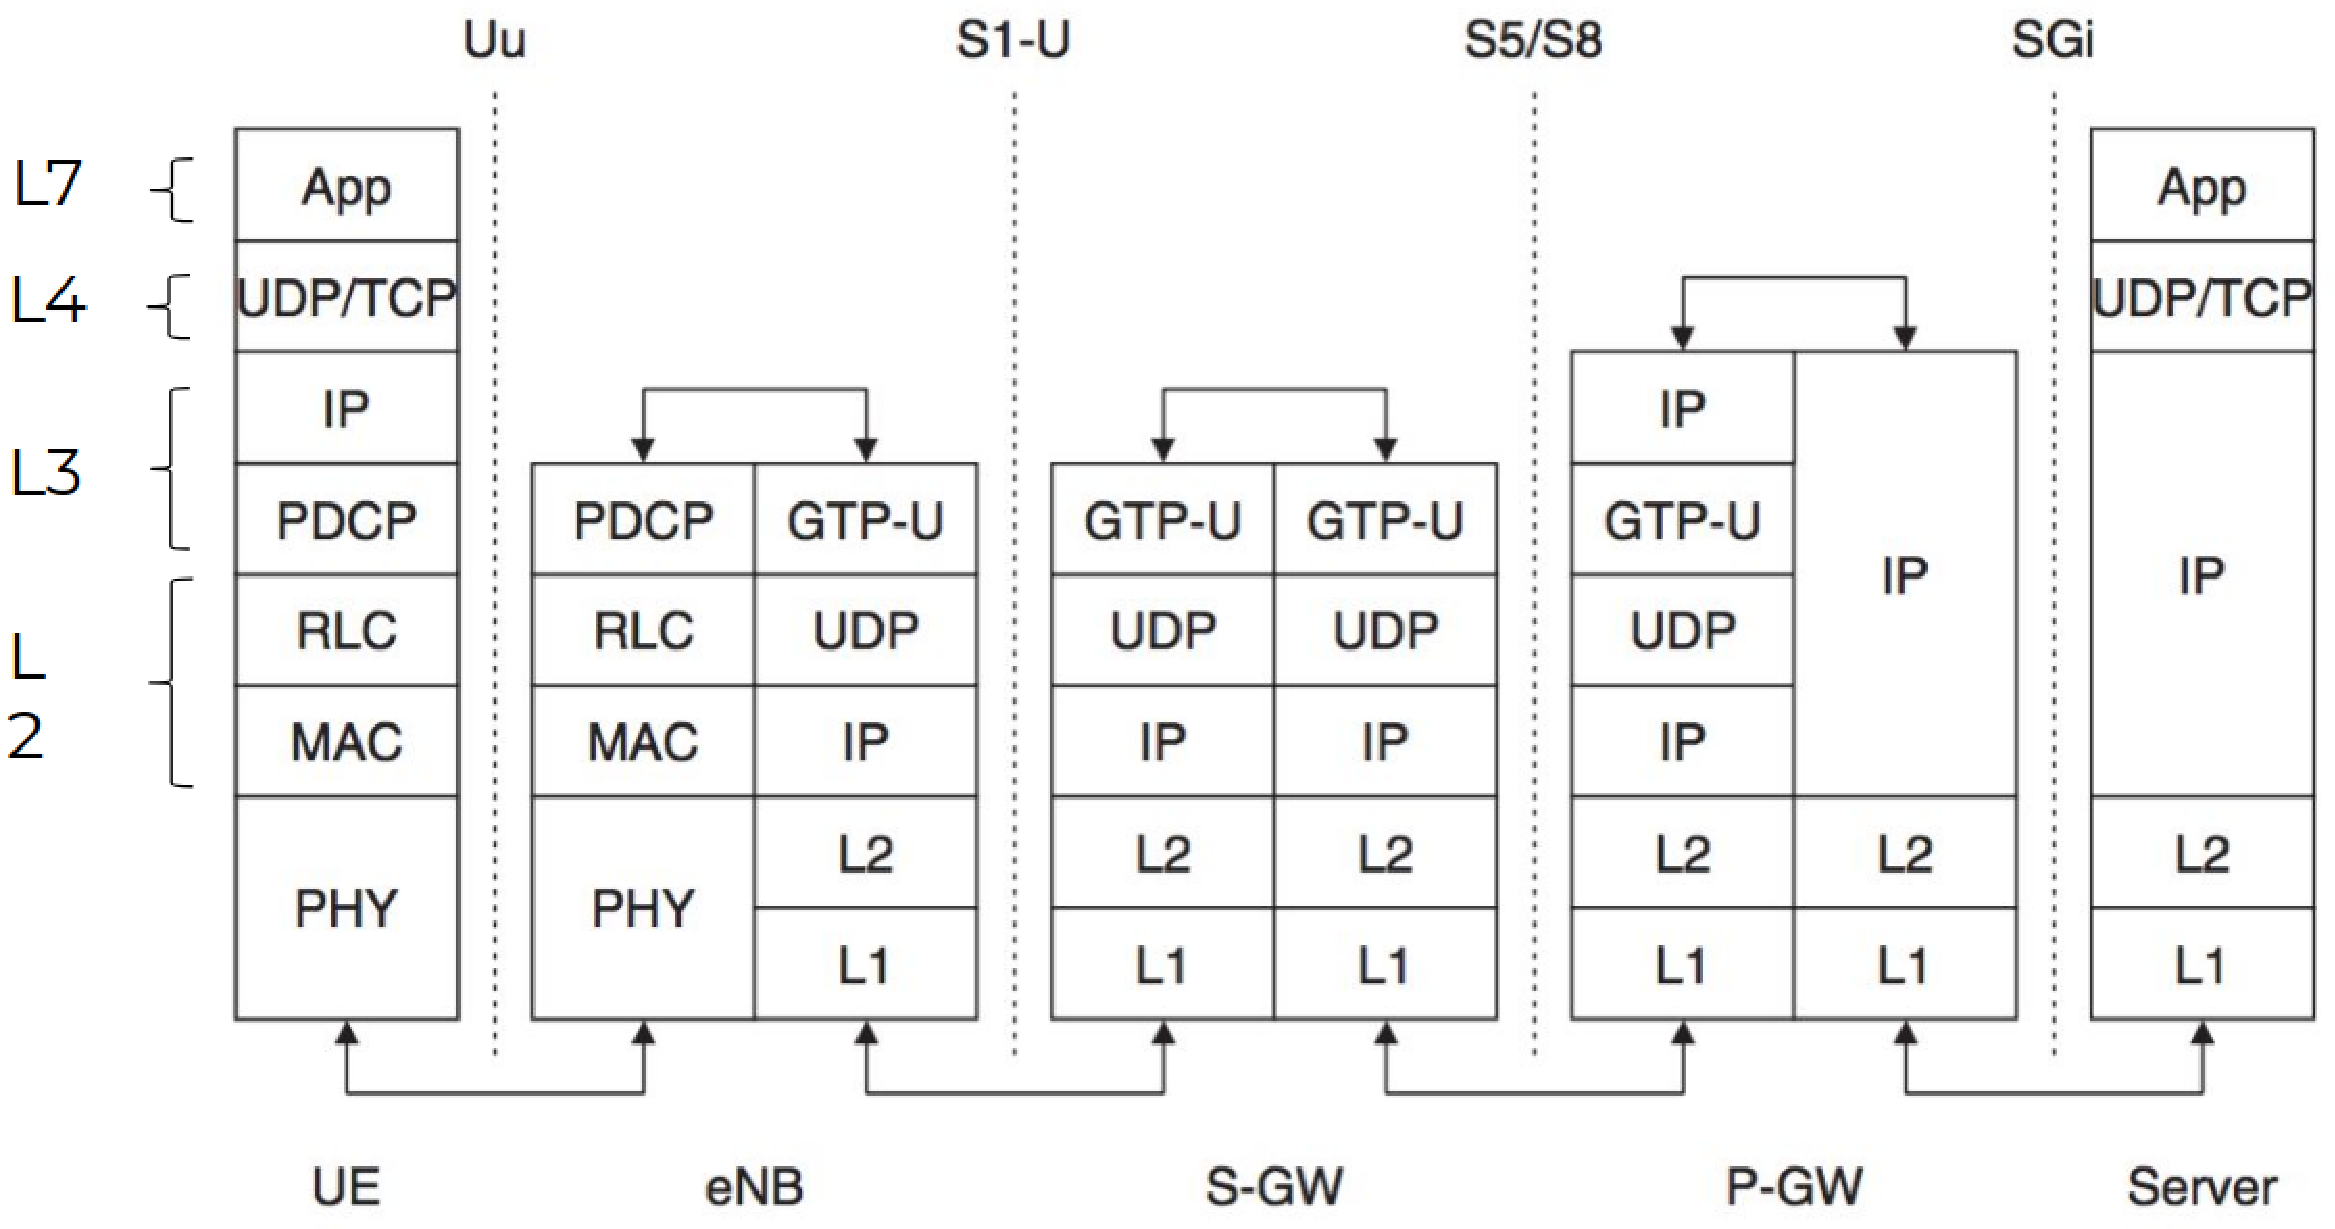
\includegraphics[width=0.9\linewidth]{img/4g/ups}
\end{center}

\paragraph{UE - eNodeB:} I primi 4 livelli sono uguali al control plane (PHY, MAC, RLC, PDCP), mentre sopra si ha uno stack IP "classico".\\

Ci sono un sacco di IP, ognuno ha il suo motivo: 
\begin{itemize}
	\item tra UE e P-GW: indirizzo IP interno, valido per tutta la connessione tra UE e P-GW, assegnato con DHCP e "nascosto" con NAT
	\item tra P-GW e server (internet, mondo esterno): indirizzo IP pubblico del P-GW, indirizzo IP pubblico del server; per "collegarlo" all'indirizzo IP interno viene usato il NAT
	\item tutti quelli sotto: indirizzi IP della rete interna dell'operatore
\end{itemize}

\newpage

\subsubsection{GPRS Tunneling Protocol GTP} 

La connessione logica tra UE e PGW è identificata da una sessione Packet Data Network (PDN).  Lo UE è libero di muoversi all'interno della rete e possiede un proprio IP unico all'interno della rete (DHCP/NAT) e mantenuto per tutta la durata della sessione. \\

eNodeB e SGW possono cambiare durante la durata della connessione. Ogni volta che un dispositivo cambia connessione bisognerebbe cambiare le tabelle di routing, ma questo sarebbe impossibile da gestire in scala, o comunque troppo dispendioso. \\

La rete è generalmente fissa (le eNodeB cambiano \textit{raramente}), l'unica parte che cambia spesso sono i collegamenti finali (i dispositivi utente).\\

Il pacchetto che parte dall'UE e gestito dall'eNodeB tramite l'interfaccia Uu è 
\begin{center}
	\begin{tabular}{l | C{1cm} | C{1cm} | C{1cm} | C{1cm} |}
		\cline{2-5}
		UE $\leftrightarrow$ eNodeB & RLC & IP & UPD/ TCP & DATA \\
		\cline{2-5}
	\end{tabular}
\end{center}

Mentre il pacchetto gestito dall'eNodeB tramite interfaccia S1-U viene incapsulato GTP:
\begin{center}
	\begin{tabular}{| C{1.5cm} | C{1.7cm} | C{2cm} | C{1.2cm} | C{1.2cm} | C{1.2cm} |}
		\multicolumn{1}{C{1.5cm}}{IP SGW} & \multicolumn{1}{C{1.7cm}}{UDP port SGW} & \multicolumn{1}{C{2cm}}{Tunnel ID (TEID)} & \multicolumn{3}{C{3.6cm}}{Pacchetto Utente \newline Incapsulamento GTP} \\
		\hline
		IP & UDP & GTP & IP & UDP/ TCP & DATA \\
		\hline
	\end{tabular}
\end{center}

Quando passa dalla eNodeB a SGW: la prossima destinazione è il PGW, quindi: 
\begin{itemize}
	\item IP SGW $\rightarrow$ IP PGW 
	\item UDP Port SGW $\rightarrow$ UDP Port PGW
	\item Il TEID prima faceva riferimento alla connessione eNodeB $\leftrightarrow$ SGW, adesso a SGW $\leftrightarrow$ PGW
\end{itemize}

\newpage

Al gateway viene rimosso l'incapsulamento NAT e GTP, prima di essere consegnato alla rete esterna.
\begin{center}
	\renewcommand{\arraystretch}{1.4}
	\begin{tabular}{| C{3cm} | C{3cm} | C{3cm} |}
		\multicolumn{3}{C{9cm}}{Pacchetto Utente \newline Rimozione incapsulamento GTP e NAT} \\
		\hline
		IP & UDP/TCP & DATA \\
		\hline
	\end{tabular}
\end{center}

L'operatore nasconde completamente la mobilità (a livello di trasferimento dati) al mondo esterno, tutti i dati passano dal P-GW.\\

\subsection{LTE EPS Bearers}

Si può astrarre a più livelli i bearer usati nella rete:

\begin{center}
	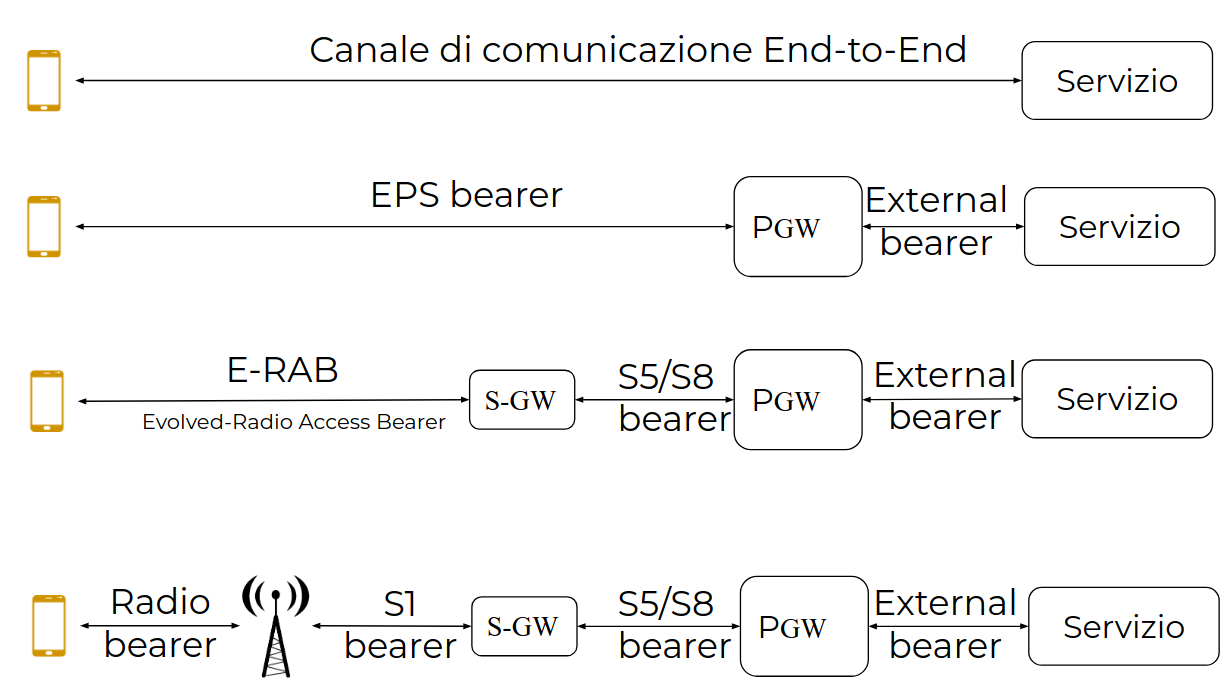
\includegraphics[width=0.85\linewidth]{img/4g/bearing}
\end{center}

Cambiare l'antenna a cui un dispositivo è collegato non richiede necessariamente di cambiare tutti i bearer: 
\begin{itemize}
	\item sicuramente cambierà il radio bearer (l'antenna a cui è collegato è diversa)
	\item cambierà l'S1 bearer se l'antenna fa parte di una nuova BS
	\item il bearer S5/S8 cambierà solo se la nuova BS fa parte di un alrto SGW
\end{itemize}

\newpage

\subsubsection{Bearer Multipli} 

Per gestire le QoS si usano \textbf{bearer multipli}. Durante la registrazione alla rete viene creato un \textbf{default bearer}, ma si può avere un \textbf{dedicated bearer}, con lo stesso indirizzo IP del default bearer da cui deriva e stesso gateway. Un'altra possibilità è avere un altro default bearer, creato dopo la registrazione, con un \textbf{nuovo P-GW}
\begin{center}
	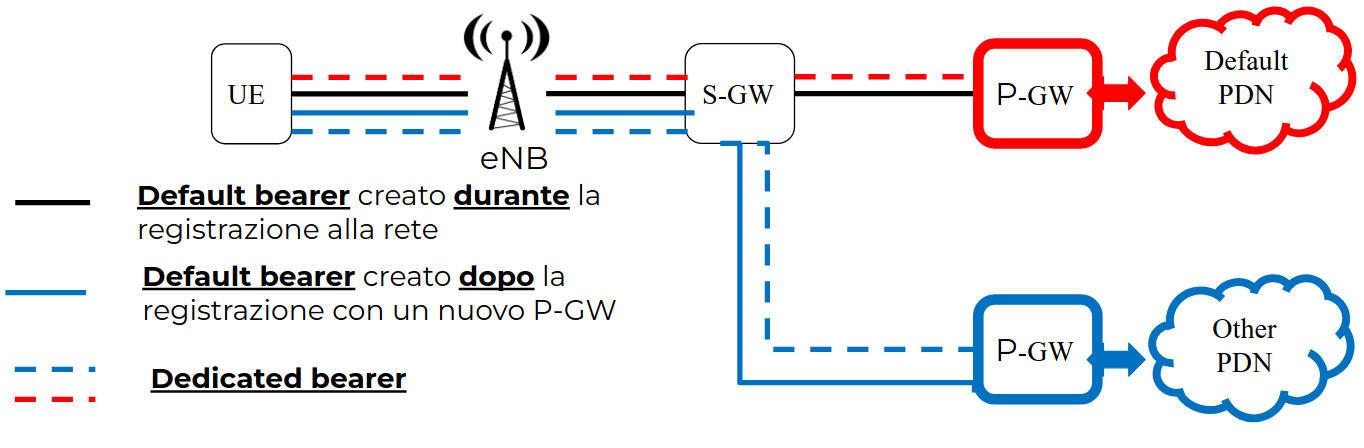
\includegraphics[width=\linewidth]{img/4g/dedicatedbearing}
\end{center}
Fino ad un massimo di 8. \\

\paragraph{Qos e EPS Bearers:} In base al servizio si può avere uno specifico \textbf{QoS Class Identifier} (QCI), con le rispettive caratteristiche: un bit rate minimo garantito oppure no (Guaranteed Bit Rate GBR vs Non-GBR), oltre che una priorità, delay e loss rate massimo. \\

I \textbf{Traffic Flow Template TFT} sono delle "mappe" istanziate al momento della connessione sul dispositivo e contengono regole generate dall'operatore telefonico per mappare un servizio sul device a una classe di QoS. Permettono di determinare la QoS che avrà un servizio (es: YouTube penso avrà QCI 7).\\

\newpage

Tabella QCI:
\begin{center}
	\resizebox{\textwidth}{!}{\begin{tabular}{c C{1.5cm} c C{1.5cm} C{2cm} C{5cm}} 
			\toprule
			\textbf{QCI} 
			& \textbf{Resource Type} 
			& \textbf{Priority} 
			& \textbf{Packet Delay Budget (ms)} 
			& \textbf{Packet Error Loss Rate} 
			& \textbf{Example Services} \\
			\midrule
			1 & GBR     & 2 & 100 & $10^{-2}$ & Conversational voice \\
			\hline
			2 & GBR     & 4 & 150 & $10^{-3}$ & Conversational video (live streaming) \\
			\hline
			3 & GBR     & 5 & 300 & $10^{-6}$ & Non-conversational video (buffered streaming) \\
			\hline
			4 & GBR     & 3 &  50 & $10^{-3}$ & Real-time gaming \\
			\hline
			5 & Non-GBR & 1 & 100 & $10^{-6}$ & IMS signaling \\
			\hline
			6 & Non-GBR & 7 & 100 & $10^{-3}$ & Voice, video (live streaming), interactive gaming \\
			\hline
			7 & Non-GBR & 6 & 300 & $10^{-6}$ & Video (buffered streaming) \\
			\hline
			8 & Non-GBR & 8 & 300 & $10^{-6}$ & TCP-based (for example, WWW, e-mail), chat, FTP, p2p file sharing, progressive video and others \\
			\hline
			9 & Non-GBR & 9 & 300 & $10^{-6}$ &  \\
			\bottomrule
	\end{tabular}}
\end{center}

%End L18